% === T18 - Sincronización de procesos ===
% David Alejandro Gonzalez Marquez
% fokerman@gmail.com
% https://github.com/fokerman/computingSystemsCourse

\documentclass[aspectratio=169]{beamer}
\usepackage{../packages}

\usepackage{keystroke}
\usepackage{menukeys} 

\title{\Huge Sincronización de procesos}
\author{David Alejandro González Márquez}
\input{../university}
\date{}

\begin{document}

\begin{frame}[plain]
    \titlepage
    \begin{textblock}{100}(30,80)
    \begin{tcolorbox}[size=small,width=\textwidth,colback={gray!30},title={}]
    \begin{center}
     \scriptsize Clase disponible en: \url{https://github.com/fokerman/computingSystemsCourse}
    \end{center}
    \end{tcolorbox}
    \end{textblock}
%     \begin{textblock}{140}(10,70)
%     \textcolor{rojo}{
%     \textbf{Atención}: La clase será grabada por el anfitrión para su posterior y eventual uso académico dentro de nuestra institución. Su participación en la clase implica brindar su consentimiento para participar en la grabación, aunque pueden mantener su video apagado.}
%     \end{textblock}
\end{frame}

\begin{frame}[t]{Sincronización de Procesos}
    \small
    En un entorno de multiprogramación, donde \textcolor{verdeuca}{\textbf{más de un proceso}} es ejecutado para resolver un problema,
    surge la necesidad de mecanismos de \textcolor{naranjauca}{\textbf{comunicación}} y \textcolor{naranjauca}{\textbf{sincronización}} entre procesos.\\
    \bigskip
    \normalsize
    \uncover<2->{
    A un conjunto de procesos que cooperan entre sí para resolver un problema los llamamos\\ \textbf{procesos cooperativos}.\\}
    \bigskip
    \small
    \uncover<2->{
    \textcolor{gray}{Por ejemplo, los múltiples procesos de un navegador web, o el conjunto de rutinas ejecutadas en paralelo por un software de procesamiento de imagenes, o incluso una IDE de desarrollo. Cualquier aplicación que utilice eficientemente los recursos del suele utilizar multiples procesos o \emph{threads}}\\}
    \bigskip
    \normalsize
    \begin{textblock}{70}(15,60)
    \uncover<3->{
    \textcolor{naranjauca}{\textbf{Mecanismos de comunicación}}\\
    \begin{itemize}
    \item[\textcolor{verdeuca}{-}] \textcolor{verdeuca}{\textbf{Memoria compartida}}
    \item[\textcolor{verdeuca}{-}] \textcolor{verdeuca}{\textbf{Pasaje de mensajes}}
    \end{itemize} }
    \end{textblock}
    \begin{textblock}{70}(85,60)
    \uncover<3->{
    \textcolor{naranjauca}{\textbf{Mecanismos de sincronización}}\\
    \begin{itemize}
    \item[\textcolor{verdeuca}{-}] \textcolor{verdeuca}{\textbf{Mutex}}
    \item[\textcolor{verdeuca}{-}] \textcolor{verdeuca}{\textbf{Semaforos}}
    \end{itemize} }
    \end{textblock}
\end{frame}

\begin{frame}[fragile,t]{Condición de carrera (\emph{race condition})}
    Supongamos el siguiente código:\\
    \begin{textblock}{70}(10,18)
    \textbf{Proceso Productor}\\
    \vspace{0.3cm}
    \footnotesize
    \verb|while(true) {                   |\\
    \color{verdeuca}
    \verb|   item = newItem();            |\\
    \vspace{0.2cm}
    \color{rojo}
    \verb|   while(count == BUFFERSIZE){};|\\
    \vspace{0.2cm}
    \color{black}
    \verb|   buffer[in] = item;           |\\
    \verb|   in = (in + 1) % BUFFERSIZE;  |\\
    \verb|   count++;                     |\\
    \verb|}                               |\\
    \end{textblock}
    \begin{textblock}{70}(80,18)
    \textbf{Proceso Consumidor}\\
    \vspace{0.3cm}
    \footnotesize
    \verb|while(true) {                    |\\
    \color{rojo}
    \verb|    while(count == 0){};         |\\
    \color{black}
    \vspace{0.2cm}
    \verb|    item = buffer[out]           |\\
    \verb|    out = (out + 1) % BUFFERSIZE;|\\
    \verb|    count--;                     |\\
    \vspace{0.2cm}
    \color{verdeuca}
    \verb|    processItem(item);           |\\
    \color{black}
    \verb|}                                |\\
    \end{textblock}
    \begin{textblock}{70}(5,60)
    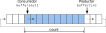
\includegraphics[scale=0.7]{img/productor_consumidor.pdf}
    \end{textblock}
    \begin{textblock}{63}(83,64)
    El productor construye items y los guarda en un buffer, mientras que el consumidor, toma los items del buffer y los procesa.
    \end{textblock}
\end{frame}

\begin{frame}[fragile,t]{Condición de carrera (\emph{race condition})}
    La cantidad de items en el \emph{buffer} es una variable compartida entre el productor y el consumidor.\\
    \medskip
    Al estar compartida, \textcolor{verdeuca}{\textbf{su edición esta sujeta a condiciones de carrera.}}\\
    \medskip
    Veamos un ejemplo en \texttt{ASM}:\\
    \begin{textblock}{70}(15,34)
    \verb|...|\\
    \verb|MOV EAX, [count]|\\
    \verb|ADD EAX, 1      |\\
    \verb|MOV [count], EAX|\\
    \verb|...|\\
    \end{textblock}
    \begin{textblock}{70}(85,34)
    \verb|...|\\
    \verb|MOV EAX, [count]|\\
    \verb|SUB EAX, 1      |\\
    \verb|MOV [count], EAX|\\
    \verb|...|\\
    \end{textblock}
    \begin{textblock}{140}(10,60)
    \small
    \textcolor{rojo}{
    El \emph{scheduler} no nos garantiza que se ejecute primero el proceso productor y luego el consumidor.\\
    Tampoco nos garantiza, \textbf{en el caso de un \emph{scheduler} apropiativo}, que se ejecuten todas las instrucciones una despues de la otra.\\}
    \medskip
    \normalsize
    \pause
    \uncover<3->{
    Por lo tanto el valor final de \texttt{count} puede \textbf{no ser el esperado}, \textcolor{naranjauca}{veamos un ejemplo.}
    }
    \end{textblock}
\end{frame}

\begin{frame}[fragile,t]{Condición de carrera (\emph{race condition})}
    \small
    Supongamos una posible ejecución \textbf{concurrente} de ambos procesos.\\
    \pause
    \begin{center}
        \begin{tabular}{|l|l|c|}
            \hline
            \multicolumn{1}{|c|}{Proceso Productor} & \multicolumn{1}{c|}{Proceso Consumidor} & Valor de \texttt{count}\\ \hline
            \texttt{...}                   &                               & \texttt{X}        \\
            \texttt{MOV EAX, [count]}      &                               & \texttt{X}        \\
            \texttt{ADD EAX, 1}            &                               & \texttt{X}        \\
                                           & \texttt{...}                  & \texttt{X}        \\
                                           & \texttt{MOV EAX, [count]}     & \texttt{X}        \\
                                           & \texttt{SUB EAX, 1}           & \texttt{X}        \\
                                           & \texttt{MOV [count], EAX}     & \texttt{X-1}      \\ 
                                           & \texttt{...}                  & \texttt{X-1}      \\
            \texttt{MOV [count], EAX}      &                               & \texttt{X+1}      \\ 
            \texttt{...}                   &                               & \texttt{X+1}      \\ \hline
        \end{tabular}
    \end{center}
    \pause
    El \textit{scheduler} puede desalojar a los procesos en \textbf{cualquier momento} de su ejecución.\\
    Por lo tanto, se puede producir un entrelazamiento (\textcolor{naranjauca}{\textbf{interleaving}}) de los procesos.\\
    \pause
    No tenemos garantías de la \textcolor{naranjauca}{\textbf{atomicidad}} de secuencias de instrucciones. \textcolor{verdeuca}{¿qué hacemos?}
\end{frame}

\begin{frame}[fragile,t]{Condición de carrera (\emph{race condition})}
    En procesos cooperativos, puede ocurrir que no todas las posibles ejecuciones entrelazadas generen resultados válidos.
    Es decir, que exista una \textbf{traza de ejecución} que genere un resultado invalido, exponiendo una \textcolor{naranjauca}{\textbf{condición de carrera}} en nuestro código.\\
    \bigskip
    \pause
    Para resolver este problema, nuestro código debe \textcolor{naranjauca}{\textbf{restringir las trazas de ejecución}} que lleven a resultados invalidos.\\
    \bigskip
    \pause
    \textcolor{verdeuca}{\textbf{¿Cómo?}}, por medio de herramientas de \textcolor{naranjauca}{\textbf{sincronización}}.\\
    \bigskip
    \pause
    Este es uno de los problemas más complejos de la Computación, y los Sistemas Operativos están no son la excepción.\\
    \medskip
    \pause
    \textcolor{gray}{
    Los diseñadores de sistemas buscan máximizar la eficiencia de sus soluciones generando múltiples procesos concurrentes,
    pero reduciendo su exposición a condiciones de carrera.
    Considerando que cuantas más restricciones agreguemos a las soluciones, más seriales serán y menos aprovecharán las ventajas de la multiprogramación.
    }
\end{frame}

\begin{frame}[fragile,t]{Sección Crítica}
    Una \textcolor{naranjauca}{\textbf{sección crítica}} es como se denomina a una parte de nuestro código que puede ser ejecutada por un solo proceso a la vez.\\
    \begin{textblock}{70}(10,24)
    Una solución para el problema de sección crítica debe garantizar:
    \begin{enumerate}
    \item \textbf{Exclusión mutua}: Si un proceso ejecuta en la sección crítica, ningún otro proceso puede ejecutar.
    \item \textbf{Avance}: La elección de que proceso va a entrar en la sección crítica se decide entre los procesos que no están en la sección crítica.
    \item \textbf{Limitación de espera}: Existe un límite de espera para poder entrar a la sección crítica.
    \end{enumerate}
    \end{textblock}
    \begin{textblock}{70}(85,24)
    \verb|...|\\
    \verb|while(true) {|\\
    \vspace{0.2cm}
    \color{verdeuca}
    \verb|    ENTRY CRITICAL SECTION|\\
    \vspace{0.2cm}
    \color{red}
    \verb|    código en la sección crítica|\\
    \vspace{0.2cm}
    \color{verdeuca}
    \verb|    EXIT CRITICAL SECTION|\\
    \vspace{0.2cm}
    \color{black}
    \verb|    resto del código|\\
    \vspace{0.2cm}
    \verb|}|\\
    \verb|...|\\
    \end{textblock}
\end{frame}

\begin{frame}{Soporte para la sincronización}
    \small
    Para poder implementar mecanismos de sección crítica en procesadores modernos.\\
    \medskip
    Es necesario conocer el \textbf{modelo de memoria} con el que opere nuestro sistema.\\
    \begin{itemize}
    \item[-] \textcolor{naranjauca}{\textbf{Consistencia fuerte}}\\
    Si un procesador modifica la memoria, el resto de los procesadores ven este cambio inmediatamente y de forma ordenada.
    \item[-] \textcolor{naranjauca}{\textbf{Consistencia debil}}\\
    Si un procesador modifica la memoria, puede que no todos los procesadores vean este cambio inmediatamente.
    \end{itemize}
    \medskip
    Dependiendo que modelo de memoria tengamos, existe soporte en \emph{hardware} para\\ \textbf{forzar la sincronización} de la memoria.\\
    \medskip
    Estos mecanismos se conocen como \textbf{barreras de memoria} (\emph{memory fences}).
\end{frame}

 
\begin{frame}[fragile]{Soporte para la sincronización}
    \small
    Existen además instrucciones especiales para implementar mecanismos de sincronización denominadas \textbf{atómicas}.\\
    \medskip
    Conceptualmente estas instrucciones realizan acciones de forma atómica.
    \medskip
    \begin{itemize}
     \item[-] \textcolor{naranjauca}{\textbf{Test And Set}}\\
    \verb|bool test_and_set(bool *target) {|\\
    \verb|    bool value = *target         |\\
    \verb|    *target = true;              |\\
    \verb|    return value                 |\\
    \verb|}                                |\\
    \item[-] \textcolor{naranjauca}{\textbf{Compare And Swap}}
    \verb|int compare_and_swap(int *value, int expected, int newValue) {|\\
    \verb|    int tmp  *value;                                          |\\
    \verb|    if (*value == expected) {                                 |\\
    \verb|        *value = new_value;                                   |\\
    \verb|    }                                                         |\\
    \verb|    return tmp;                                               |\\
    \verb|}                                                             |\\
    \end{itemize}
\end{frame}

\begin{frame}[fragile,t]{Exclusión mutua (\texttt{mutex} - \emph{\textbf{mut}ual \textbf{ex}clusion})}
    Utilizando estas instrucciones podemos implementar un mecanismo de sección crítica garantizando la exclusión mutua.\\
    \small
    \bigskip
    \verb|do {                              |\\
    \vspace{0.2cm}
    \color{verdeuca}
    \verb|  while(test_and_set(&lock)){};   |\\
    \vspace{0.2cm}
    \color{red}
    \verb|  CODIGO EN LA SECCION CRITICA    |\\
    \color{black}
    \vspace{0.2cm}
    \color{verdeuca}
    \verb|  lock = false;                   |\\
    \color{black}
    \vspace{0.2cm}
    \verb|  RESTO DEL CODIGO                |\\
    \vspace{0.2cm}
    \verb|} while(true);                    |
    \begin{textblock}{65}(75,24)
    \begin{tcolorbox}[size=small,width=\textwidth,title={Candados (\emph{locks})}]
    Variables \emph{booleanas} compartidas.\vspace{0.2cm}\\
    \textbf{Para tomar el candado:}\vspace{0.2cm}\\
    Si el candado está en \texttt{true}, espero a que cambie en \texttt{false}.\\
    Si el candado está en \texttt{false}, lo cambio a \texttt{true} para que nadie me interrumpa.\vspace{0.2cm}\\
    \textbf{Para liberar el candado:}\vspace{0.2cm}\\
    Cuando termino cambio el candado a \texttt{false}, para que otro lo pueda usar.
    \end{tcolorbox}
    \end{textblock}
\end{frame}

%     \texttt{acquire()}
%     \texttt{release()}
%     \begin{verbatim}
%     acquire() {
%         while(!available){};
%         available = false;
%     }
%     \end{verbatim}
% 
%     \begin{verbatim}
%     release() {
%         available = true;
%     }
%     \end{verbatim}
%     
%     \begin{verbatim}
%     ...
%     while(true) {
%     
%         CÓDIGO NO CRITICO
%         
%         acquire();
%     
%         CÓDIGO EN LA SECCIÓN CRITICA
%     
%         release();
%         
%         CÓDIGO NO CRITICO
%     }
%     ...
%     \end{verbatim}

\begin{frame}{Spin Locks}
    La desventaja de la implementación anterior es que para obtener el \emph{lock} estamos realizando una \textbf{espera activa} (busy waiting).\\
    \bigskip
    \textcolor{verdeuca}{\textbf{Estamos utilizando la CPU para no hacer nada productivo, solo esperar.\\
    Impidiendo además que otros procesos puedan acceder al procesador.\\}}
    \bigskip
    \pause
    Sin embargo, los \emph{spin locks} tienen ventajas, ya que no tenemos que realizar\\ ningún cambio de contexto.\\
    \bigskip
    En determinados casos, cuando el tiempo de espera es muy corto y los eventos de sincronización se dan muy seguidos.\\
    \textcolor{naranjauca}{La solución de \emph{spin locks} es la más eficiente.}
    \begin{center}
    \pause
    \textcolor{verdeuca}{\textbf{¿y qué tal sí el sistema espera por nosotros?}}
    \end{center}
\end{frame}

\begin{frame}[fragile,t]{Semáforos}
Un semáforo es una variable entera que solo puede ser modificada por las operaciones:
\begin{itemize}
 \item[-] \textcolor{naranjauca}{\texttt{signal()}}: Incrementa el valor del semáforo en 1.\\
 \vspace{0.2cm}
    \verb|    signal(int* S) { |\\
    \verb|      (*S)++;        |\\
    \verb|    }                |\\ 
 \vspace{0.2cm}
 \item[-] \textcolor{naranjauca}{\texttt{wait()}}: Espera hasta que el valor del semáforo sea menor o igual a 0,\\
 \hspace{1.35cm}y luego decrementa el valor del semáforo en 1.\\
 \vspace{0.2cm}
    \verb|    wait(int* S) {   |\\
    \verb|      while(*S<=0){};|\\
    \verb|      (*S)--;        |\\ 
    \verb|    }                |\\
\end{itemize}
Estas dos primitivas deben ser ejecutadas de forma \textbf{atómica} por el sistema operativo.\\
\textcolor{naranjauca}{Pero como las implementamos para no hacer una espera activa.}
\end{frame}

\begin{frame}[fragile,t]{Implementación de Semáforos}
    Se declara a nivel del sistema operativo la estructura del semáforo.\\
    \bigskip
    \footnotesize
    \verb|struct semaphore {       |\\
    \verb|    int value;           |\\
    \verb|    struct process *list;|\\
    \verb|}                        |\\
    \begin{textblock}{65}(10,40) 
    \footnotesize
    \verb|void wait(semaphore* s) {               |\\
    \verb|    s->value--;                         |\\
    \verb|    if(s->value < 0) {                  |\\
    \verb|        addList(s->list,current_process)|\\
    \verb|        sleep();                        |\\
    \verb|    }                                   |\\
    \verb|}                                       |\\
    \bigskip
    Decrementa el semáforo y consulta su estado.\\
    Si debe esperar, agrega al proceso a una lista\\
    de procesos en espera para adquirir el semáforo.
    \end{textblock}
    \begin{textblock}{65}(75,40)
    \footnotesize
    \verb|void signal(semaphore* s) {            |\\
    \verb|    s->value++;                        |\\
    \verb|    if(s->value <= 0) {                |\\
    \verb|        process = removeList(s->list)  |\\
    \verb|        wakeup(process);               |\\
    \verb|    }                                  |\\
    \verb|}                                      |\\
    \bigskip
    Incrementa el semáforo, compara si hay procesos\\
    esperando, en cuyo caso los despierta.
    \end{textblock}
\end{frame}

\begin{frame}[fragile,t]{Ejemplo de uso de Semáforos}
    El uso de semáforos permite resolver diferentes problemas de sincronización.\\
    \medskip
    En el ejemplo, el proceso A ejecuta \texttt{CODE} \texttt{A} y luego llama a \texttt{signal}.\\
    \medskip
    Por otro lado, el proceso B llama \texttt{wait} y luego ejecuta \texttt{CODE} \texttt{B}.\\
    \begin{textblock}{70}(15,34)
    \textbf{Proceso A}\\
    \medskip
    \verb|...|\\
    \verb|CODE A|\\
    \verb|signal(sync)|\\
    \verb|...|\\
    \end{textblock}
    \begin{textblock}{70}(85,34)
    \textbf{Proceso B}\\
    \medskip
    \verb|...|\\
    \verb|wait(sync)|\\
    \verb|CODE B|\\
    \verb|...|\\
    \end{textblock}
    \begin{textblock}{140}(10,65)
    \uncover<2->{
    Esto garantiza que \texttt{CODE} \texttt{B} se ejecute después de \texttt{CODE} \texttt{A}.
    }
    \end{textblock}
\end{frame}

\begin{frame}[t]{Interbloqueo (\textit{deadlock})}
    Cualquier mecanismo de sincronización donde múltiples procesos esperen por un recurso nos puede llevar a una situación de \emph{deadlock}.
    En particular el uso de semáforos.\\
    \bigskip
    Cuando conjunto de procesos se quedan simultáneamente esperando que ocurra un evento, que los mismos procesos que esperan deben generar, entonces estamos en un \textcolor{naranjauca}{\textbf{deadlock}}.\\
    \bigskip
    \textcolor{gray}{Ejemplo:\\}
    \only<2->{\hspace{30mm} A no continúa hasta que B no envíe un \texttt{signal()}.\\}
    \only<3->{\hspace{30mm} Pero B no continúa hasta que C no envíe un \texttt{signal()}.\\}
    \only<4->{\hspace{30mm} Pero C no continúa hasta que D no envíe un \texttt{signal()}.\\}
    \only<5->{\hspace{30mm} Pero D no continúa hasta que A no envíe un \texttt{signal()}.\\}    
    \bigskip    
    \only<6->{También se puede dar la situación en que un proceso espera indefinidamente.\\
    Esta situación se conoce como \textcolor{naranjauca}{\textbf{inanición}} o \textcolor{naranjauca}{\textbf{\textit{starvation}}}.}
\end{frame}

\begin{frame}
    \frametitle{\textit{Deadlock}: ejemplo gráfico}
    \begin{center}
        \includegraphics[scale=0.3]{img/deadlock_traffic.jpeg}
    \end{center}
\end{frame}

\begin{frame}
    \frametitle{\textit{Deadlock}: ejemplo gráfico}
    \begin{center}
        \includegraphics[scale=0.4]{img/deadlock_spiderman.jpeg}
    \end{center}
\end{frame}

\begin{frame}[t]{Barreras o \textit{barriers}}
    \small
    Existen problemas donde es necesario varios procesos se sincronicen en un punto del programa.\\
    \textcolor{verdeuca}{El problema de sincronización consiste en hacer esperar a todos los procesos
    y una vez que todos llegaron, pueden continuar.\\}
    \bigskip
    \only<2->{Para estos casos, existe un mecanismo de sincronización distinto conocido
    como \textcolor{naranjauca}{\textbf{barrera}} o \textcolor{naranjauca}{\textbf{\textit{barrier}}}.}
    
    \begin{textblock}{140}(15,40) \only<3->{\includegraphics[scale=1.5]{img/barrier-layer1.pdf}} \end{textblock}
    \begin{textblock}{140}(60,40) \only<4->{\includegraphics[scale=1.5]{img/barrier-layer2.pdf}} \end{textblock}
    \begin{textblock}{140}(105,40)\only<5->{\includegraphics[scale=1.5]{img/barrier-layer3.pdf}} \end{textblock}
\end{frame}

\begin{frame}{Problemas clásicos de sincronización}
    Existen varios problemas teóricos clásicos sobre sincronización de procesos:\\
    \bigskip
    \begin{itemize} 
        \item Productores-consumidores.
        \item Los lectores y escritores.
        \item La cena de los filósofos.
        \item El barbero dormilón.
    \end{itemize}
    \bigskip
    A quienes estén interesados en profundizar sobre el tema,\\ les recomendamos leerlos de la bibliografía.
\end{frame}

\begin{frame}[fragile]
    \frametitle{Bibliografía}
    \begin{itemize}
        \setlength\itemsep{0.5cm}
        \item[-] \small Silberschatz, ``Fundamentos de Sistemas Operativos'', 7ma Edición, 2006.\\
        \begin{itemize}
            \item \textbf{Capítulo 6 - Sincronización de procesos}, páginas 171-186 y 161-165
        \end{itemize}
        \item[-] \small Tanenbaum, ``Modern Operating Systems'', 4th Edition, 2015.\\
        \begin{itemize}
            \item \textbf{Chapter 2 - Processes and Threads}
            \begin{itemize}
                \item 2.3 Interprocess communication - Páginas 119-137 y 146-148
                \item 2.4 Classical IPC problems - Páginas 167-172
            \end{itemize}
        \end{itemize}
    \end{itemize}
\end{frame}

\begin{frame}[plain]
    \begin{center}
    \vspace{2cm}
    \huge ¡Gracias!\\
    \vspace{2cm}
    \normalsize Recuerden leer los comentarios adjuntos\\ en cada clase por aclaraciones.
    \end{center}
\end{frame}

\end{document}

